% Alt master file to be processed with Pandoc

% Documentclass
\documentclass[9pt, twocolumn, lineno]{setting/pi/pi-article}

% Metadata
% !TEX root = ../manuscript.tex

%%%%%%%%%%%%%%%%%%%%%%%%%%%%%%%%%%%%%%%%%%%%%%%%%%%%%%%%%%%%%%%%%%%%%
%% Title
%% -----
%%%%%%%%%%%%%%%%%%%%%%%%%%%%%%%%%%%%%%%%%%%%%%%%%%%%%%%%%%%%%%%%%%%%%

\newcommand{\pubtitle}{This is the paper title}

%%%%%%%%%%%%%%%%%%%%%%%%%%%%%%%%%%%%%%%%%%%%%%%%%%%%%%%%%%%%%%%%%%%%%
%% Metadata
%% --------
%%%%%%%%%%%%%%%%%%%%%%%%%%%%%%%%%%%%%%%%%%%%%%%%%%%%%%%%%%%%%%%%%%%%%

\newcommand{\pubauthA}{Paul Iacomi}
\newcommand{\pubauthB}{Someone Else}
\newcommand{\pubauthC}{}
\newcommand{\pubauthD}{}
\newcommand{\pubauthE}{}
\newcommand{\pubauthF}{}
\newcommand{\pubauthG}{}
\newcommand{\pubauthH}{}
\newcommand{\pubauthI}{}

\newcommand{\pubaddrA}{%
Aix-Marseille Université, CNRS, MADIREL UMR 7246, 13397 Marseille, France}
\newcommand{\pubaddrB}{%
Long address from someone else or other affiliation
}
\newcommand{\pubaddrC}{%
}
\newcommand{\pubaddrD}{%
}

\newcommand{\pubemail}{iacomi.paul@email.com}

%%%%%%%%%%%%%%%%%%%%%%%%%%%%%%%%%%%%%%%%%%%%%%%%%%%%%%%%%%%%%%%%%%%%%
%% Keywords
%% --------
%%%%%%%%%%%%%%%%%%%%%%%%%%%%%%%%%%%%%%%%%%%%%%%%%%%%%%%%%%%%%%%%%%%%%
\newcommand{\pubkeywords}{%
Keyword 1 \sep Keyword 2 \sep Keyword 3}

% Preamble
% !TEX root = ../../manuscript.tex

%%%%%%%%%%%%%%%%%%%%%%%%%%%%%%%%%%%%%%%%%%%%%%%%%%%%%%%%%%%%%%%%%%%%%
%%%%%%%%%%%%%%%%%%%%%%%%%%%%%%%%%%%%%%%%%%%%%%%%%%%%%%%%%%%%%%%%%%%%%
%% In an PI manuscript the preamble contains
%%      - paper title
%%      - paper metadata
%%      - paper abstract
%%      - paper keywords
%%      - vertical space adjustment between text and abstract
%%%%%%%%%%%%%%%%%%%%%%%%%%%%%%%%%%%%%%%%%%%%%%%%%%%%%%%%%%%%%%%%%%%%%
%%%%%%%%%%%%%%%%%%%%%%%%%%%%%%%%%%%%%%%%%%%%%%%%%%%%%%%%%%%%%%%%%%%%%


%%%%%%%%%%%%%%%%%%%%%%%%%%%%%%%%%%%%%%%%%%%%%%%%%%%%%%%%%%%%%%%%%%%%%
%% Title
%% -----
%%%%%%%%%%%%%%%%%%%%%%%%%%%%%%%%%%%%%%%%%%%%%%%%%%%%%%%%%%%%%%%%%%%%%
\title{\pubtitle{}}

%%%%%%%%%%%%%%%%%%%%%%%%%%%%%%%%%%%%%%%%%%%%%%%%%%%%%%%%%%%%%%%%%%%%%
%% Meta-data block
%% ---------------
%%%%%%%%%%%%%%%%%%%%%%%%%%%%%%%%%%%%%%%%%%%%%%%%%%%%%%%%%%%%%%%%%%%%%

\author[a, *]{\pubauthA{}~\protect\orcid{\orcidA}\textsuperscript{\dag,~}}
\author[a, b]{\pubauthB{}~\protect\orcid{\orcidB}\textsuperscript{\dag,~}}
\leadauthor{P. Iacomi}
\contact{\pubemail{}}
\equalcontrib{}

\affil[a]{\pubaddrA{}}
\affil[b]{\pubaddrB{}}

\pubdoi{10.0000/xxxxxxxxxxx}

%%%%%%%%%%%%%%%%%%%%%%%%%%%%%%%%%%%%%%%%%%%%%%%%%%%%%%%%%%%%%%%%%%%%%
%% Abstract
%% --------
%%%%%%%%%%%%%%%%%%%%%%%%%%%%%%%%%%%%%%%%%%%%%%%%%%%%%%%%%%%%%%%%%%%%%

\begin{abstract}
    % !TEX root = ../manuscript.tex

\lipsum[1]{}%
\end{abstract}

%%%%%%%%%%%%%%%%%%%%%%%%%%%%%%%%%%%%%%%%%%%%%%%%%%%%%%%%%%%%%%%%%%%%%
%% Keywords
%% --------
%%%%%%%%%%%%%%%%%%%%%%%%%%%%%%%%%%%%%%%%%%%%%%%%%%%%%%%%%%%%%%%%%%%%%

\keywords{\pubkeywords{}}

%%%%%%%%%%%%%%%%%%%%%%%%%%%%%%%%%%%%%%%%%%%%%%%%%%%%%%%%%%%%%%%%%%%%%
%% Adjusting vertical space
%% ------------------------
%%%%%%%%%%%%%%%%%%%%%%%%%%%%%%%%%%%%%%%%%%%%%%%%%%%%%%%%%%%%%%%%%%%%%

% \verticaladjustment{0pt}


% Graphics
\graphicspath{ {figs/} }
\DeclareGraphicsExtensions{.png}

% Fixes for Pandoc conversion
%
% Chemical equations become plain math
\renewcommand{\ce}[1]{\(#1\)}

% SIrange becomes SIRange (TODO remove next pandoc version)
\renewcommand{\SIrange}[3]{\SIRange{#1}{#2}{#3}}

% si{} becomes blank SI{}{} (TODO remove next pandoc version)
\renewcommand{\si}[1]{\SI{}{#1}}

% copyright added
\renewcommand{\textcopyright}[0]{©}

% angstrom added
\renewcommand{\angstrom}[0]{Å}

% using cleveref as it is picked up by pandoc
\renewcommand{\autoref}[1]{\cref{#1}}

% making the figure* environment a regular figure environment
\newenvironment{figure2col}{\begin{figure}}{\end{figure}}

% SI
\externaldocument{manuscript-SI}

%%%%%%%%%%%%%%%%%%%%%%%%%%%%%%%%%%%%%%%%%%%%%%%%%%%%%%%%%%%%%%%%%%%%%

\begin{document}

% Doc input
% !TEX root = ../../manuscript.tex

%%%%%%%%%%%%%%%%%%%%%%%%%%%%%%%%%%%%%%%%%%%%%%%%%%%%%%%%%%%%%%%%%%%%%
%%%%%%%%%%%%%%%%%%%%%%%%%%%%%%%%%%%%%%%%%%%%%%%%%%%%%%%%%%%%%%%%%%%%%
%% In an PI manuscript, the document insert contains
%%      - the maketitle command
%%      - settings for naming hyperref hyperlinks
%%      - the footnote SI note
%%%%%%%%%%%%%%%%%%%%%%%%%%%%%%%%%%%%%%%%%%%%%%%%%%%%%%%%%%%%%%%%%%%%%
%%%%%%%%%%%%%%%%%%%%%%%%%%%%%%%%%%%%%%%%%%%%%%%%%%%%%%%%%%%%%%%%%%%%%

\maketitle

\makeatletter\if@switchSI\else
\footnotetext{%
Electronic Supplementary Information (ESI) available:
one PDF file with all referenced supporting information.
}
\fi\makeatother

% Content
% !TEX root = ../manuscript.tex

% !TEX root = ../manuscript.tex

%%%%%%%%%%%%%%%%%%%%%%%%%%%%%%%%%%%%%%%%%%%%%%%%%%%%%%%%%%%%%%%%%%%%%
%% Start the main part of the manuscript here.
%%%%%%%%%%%%%%%%%%%%%%%%%%%%%%%%%%%%%%%%%%%%%%%%%%%%%%%%%%%%%%%%%%%%%

\section{Introduction}

Herein we refer to a table (\cref{tbl:example-table}), but also to a figure
(\cref{fig:caption-1}) or a latter equation (\cref{eq:example}). Finally,
figures (\cref{fig:caption-si}) from the SI can also be referenced. We can add
citations as well \citep{example}. Units are inserted with the help of
\texttt{siunitx}. We can have some standard data \SI{40}{\kilo\joule\per\mol} or
ranges such as \SIrange{20}{30}{\angstrom}. Finally simple unit typesetting is
also possible \si{\mega\hertz\per\kilo\pascal}. 

Chemistry is included by referring to the \texttt{mhchem} package. Simple
molecules like \ce{N2} and \ce{C2H4} should be easy to include. More complex
formula typesetting is possible too: \ce{^{13}C} NMR, \ce{CaCl2 * 12H2O} and
\ce{Fe^{II}Fe^{III}2O4}.

Equations are in a standard Latex \texttt{equation} environment.

\begin{equation}\label{eq:example}
    e^{i\pi} + 1 = 0
\end{equation}

\lipsum[1-4]{}
% !TEX root = ../manuscript.tex

%%%%%%%%%%%%%%%%%%%%%%%%%%%%%%%%%%%%%%%%%%%%%%%%%%%%%%%%%%%%%%%%%%%%%
%% Materials and methods.
%%%%%%%%%%%%%%%%%%%%%%%%%%%%%%%%%%%%%%%%%%%%%%%%%%%%%%%%%%%%%%%%%%%%%

\section{Materials and methods}

\lipsum[2-5]{}

\begin{table}[htb]
    \caption{%
        An example table, with caption on top.
    }\label{tbl:example-table}
    \centering
    \begin{tabular}{ccc}
        \toprule
        Head 1 & Head 2 & Head 3 \\
        \midrule
        Content 1 & Content 2 & Long Content 2 \\
        Content 4 & Content 5 & Even Longer Content 6 \\
        \midrule
        \multicolumn{3}{l}{* Multicolmns are also possible}\\
        \bottomrule
    \end{tabular}
\end{table}

\lipsum[1-9]{}
% !TEX root = ../manuscript.tex

%%%%%%%%%%%%%%%%%%%%%%%%%%%%%%%%%%%%%%%%%%%%%%%%%%%%%%%%%%%%%%%%%%%%%
%% Results and discussion here.
%%%%%%%%%%%%%%%%%%%%%%%%%%%%%%%%%%%%%%%%%%%%%%%%%%%%%%%%%%%%%%%%%%%%%

\section{Results and discussion}

\begin{figure}[htb]
    \centering
    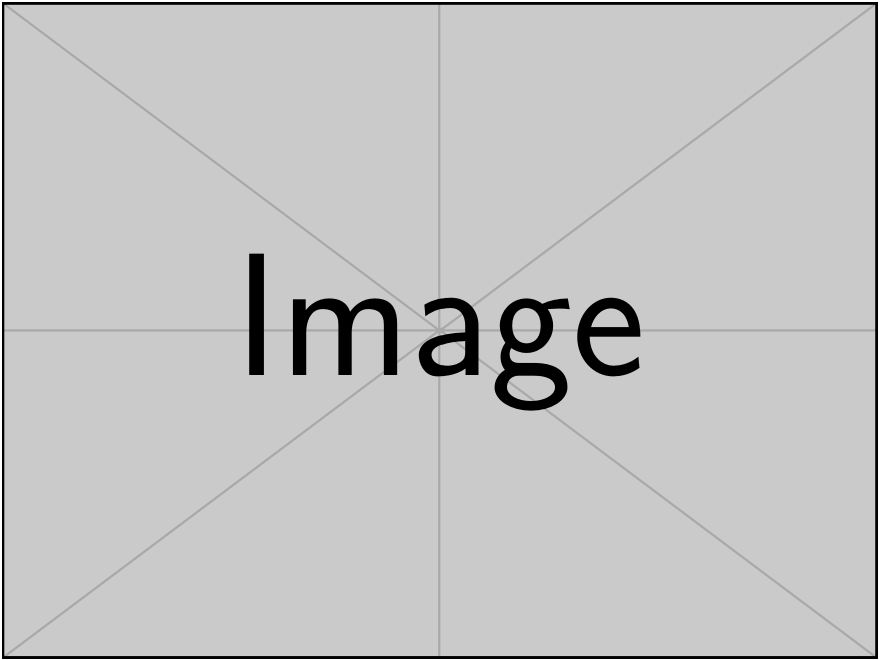
\includegraphics[width=0.9\linewidth]{example-image}
    \caption{%
        Example small figure and its caption.
    }\label{fig:caption-1}
\end{figure}

\lipsum[1-6]{}

\begin{figure*}[htb]
    \centering
    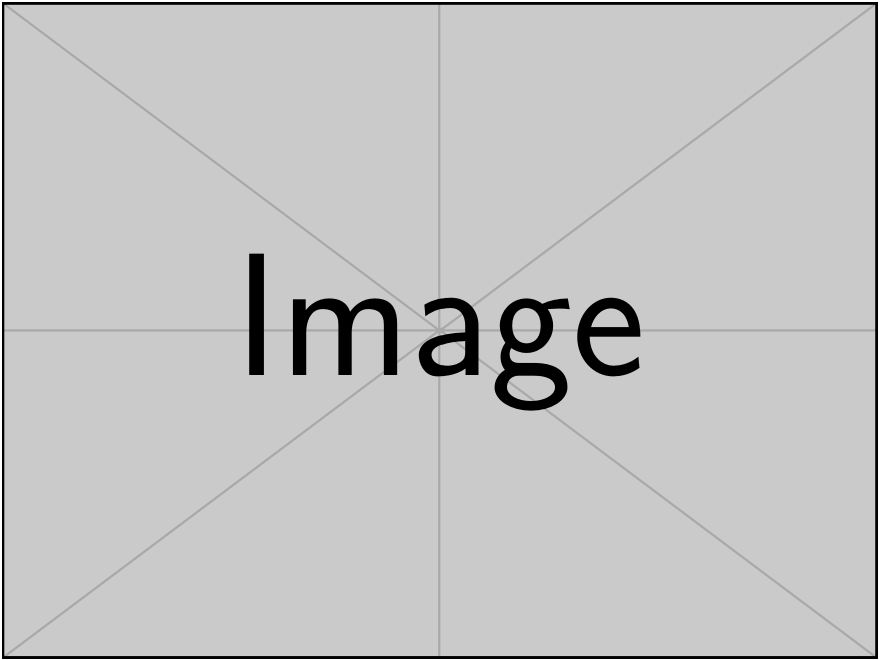
\includegraphics[width=0.9\linewidth]{example-image}
    \caption{%
        Example twocolumn large figure.
    }\label{fig:caption-2}
\end{figure*}

\lipsum[2-4]{}
% !TEX root = ../manuscript.tex

%%%%%%%%%%%%%%%%%%%%%%%%%%%%%%%%%%%%%%%%%%%%%%%%%%%%%%%%%%%%%%%%%%%%%
%% Conclusions here.
%%%%%%%%%%%%%%%%%%%%%%%%%%%%%%%%%%%%%%%%%%%%%%%%%%%%%%%%%%%%%%%%%%%%%

\section{Conclusions}

\lipsum[4-5]{}


% Doc end input
\section*{Acknowledgements}
% !TEX root = ../manuscript.tex

%%%%%%%%%%%%%%%%%%%%%%%%%%%%%%%%%%%%%%%%%%%%%%%%%%%%%%%%%%%%%%%%%%%%%
%% Acknowledgements here.
%%%%%%%%%%%%%%%%%%%%%%%%%%%%%%%%%%%%%%%%%%%%%%%%%%%%%%%%%%%%%%%%%%%%%

\lipsum[2]{}


\section*{Author contributions}
% !TEX root = ../manuscript.tex

%%%%%%%%%%%%%%%%%%%%%%%%%%%%%%%%%%%%%%%%%%%%%%%%%%%%%%%%%%%%%%%%%%%%%
%% Author contributions here.
%%%%%%%%%%%%%%%%%%%%%%%%%%%%%%%%%%%%%%%%%%%%%%%%%%%%%%%%%%%%%%%%%%%%%

\lipsum[10]{}


% SI at the end
% !TEX root = ../../manuscript-SI.tex

\section{Supplementary Information}

\subsection{SI section 1}

Here is a citation. \citep{example}

\lipsum[1]{}

\begin{figure}[htb]
    \centering
    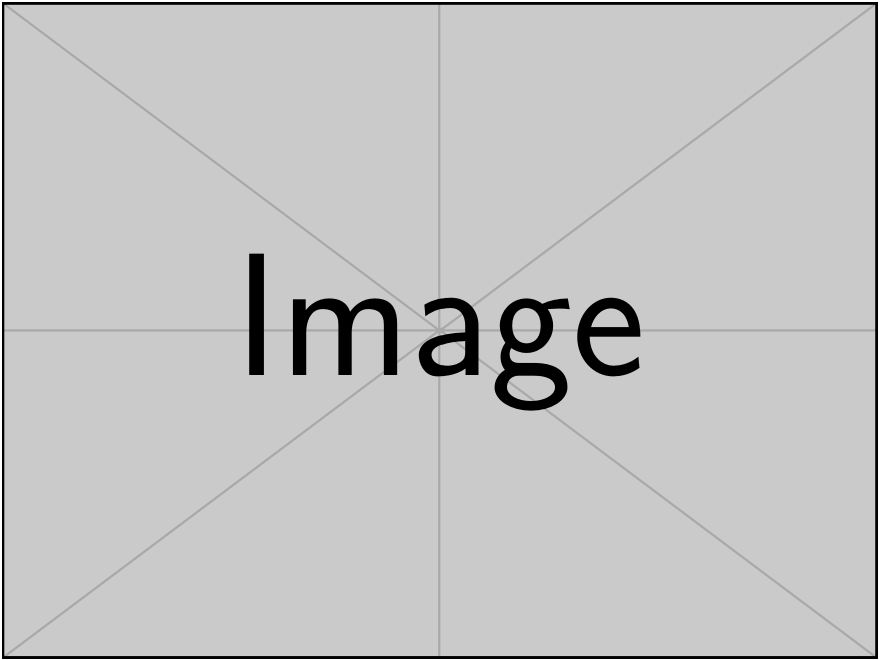
\includegraphics[width=0.9\linewidth]{example-image}
    \caption{%
        Example caption.
    }\label{fig:caption-si}
\end{figure}

\lipsum[5]{}

\subsection{SI section 2}

We are referring to previous \cref{fig:caption-si}.

\lipsum[5]{}


\section*{References}
\bibliography{refs/biblio}

% End doc
\end{document}
%%%%%%%%%%%%%%%%%%%%%%%%%%%%%%%%%%%%%%%%%%%%%%%%%%%%%%%%%%%%%%%%%%%%%